\section{Objects and event selection}
\label{sec:obj_sel}

{\color{red} This section already has been copy-pasted to common note and had been updated there.}

The response to particles traversing and interacting with the CMS detector volume is converted into a collection of physics objects using the Particle Flow algorithm {\color{red} REF}.  The signal topology of this search is characterized by a single isolated electron or muon, four or more jets, one of which is $b$-tagged, and lage \MET.  The following selection is used to isolate this type of event in data.  

\subsection{Trigger}
\label{sec:obj_sel:trigger}     

The analysis triggers are single lepton triggers, listed in table {\color{red} REF}. The plateau in trigger efficiency drives the choice of lepton \pt.  The efficiency of the triggers can be seen in figure {\color{red} NEED FIGURE}. A scale factor is applied to the simulation to account for the difference in efficiency with respect to the measured data {\color{red} NEED SF SFIGURE}.

\subsection{Lepton Selection}
\label{sec:obj_sel:lepton_sel}

This analysis selects one and only one high \pt, isolated electron or muon.  There are two sets of criteria used to classify the lepton as either a \textit{selected} or \textit{veto} lepton, which are described tables \ref{tab:el_selection} and \ref{tab:mu_selection}.

\begin{table}
\begin{center}
\caption{\label{tab:el_selection} Selection cuts for electrons selected for use in the analysis, or veto the event if found as an additional lepton}
\begin{tabular}{ l | c | c }
\hline
        & \textit{selected} & \textit{veto} \\ \hline
    \pt & 40 \GeV & 5 \GeV \\
    $\eta$ & 2.1 & 2.4 \\
    POG ID & Medium & Veto \\
    mini relative isolation & 0.1 & 0.2 \\
\hline
\end{tabular}
\end{center}
\end{table}


\begin{table}
\begin{center}
\caption{\label{tab:mu_selection} Selection cuts for muons selected for use in the analysis, or veto the event if found as an additional lepton}
\begin{tabular}{ l | c | c }
\hline
        & \textit{selected} & \textit{veto} \\ \hline
    \pt & 30 \GeV & 5 \GeV \\
    $|\eta|$ & 2.1 & 2.4 \\
    POG ID & Medium & Loose \\
    mini relative isolation & 0.1 & 0.2 \\
\hline
\end{tabular}
\end{center}
\end{table}

Mini relative isolation is defined as the sum of \pt of particle flow candidates, within a cone size which varies with the \pt of object for which this value is being calcualted.  The cone size begins at 0.2 for $\pt<50$, then is inversly proportional to the \pt from $50<\pt<200$, given by 10.0/\pt, and finally is a constant size of 0.05 for $\pt>200$.  This is to take advantage of the characteristic signature of the signal, which features very high \pt leptons that are well isolated.  By allowing the cone size to shrink with increased \pt, fewer signal events are vetoed due to pileup or nearby jet fragments.  
Pileup mitigation on the calculation is performed via a \textit{delta-beta} correction, which consists of all of the \pt from pions within the cone computed above.  
The POG IDs are a series of qualtiy cuts on the lepton reconstruction.  The following table describes the cuts used for electrons {\color{red} Need This?}


\subsubsection{Jet Selection}
\label{sec:obj_sel:jet_sel}

Jets are reconstructed using the anti-kt algorithm {\color{red} RED}, with a distance parameter of 0.4.  The selection requires at least three jets meeting the criteria described in table \ref{tab:jets_selection}.

\begin{table}
\begin{center}
\caption{\label{tab:jets_selection} Selection cuts for jets used in the analysis}
\begin{tabular}{ l | c }
\hline
  \pt & 30 \GeV \\
  $\eta$ & 2.4 \\
  ${\Delta}R(selected~lepton,~jet)$ & $>$0.4 \\
  Number of Constituents & $>$2  \\
  Neutral EM Fraction & $<$0.99 \\
  Neutral Hadron Fraction & $<$0.99 \\
  Charged Multiplicity & $\ge$1 \\
  Charged Hadron Fraction & $\ge1^{-6}$ \\
  Charged EM Fraction & $<$0.99 \\
\hline
\end{tabular}
\end{center}
\end{table}

Additionally, at least one jet is required to pass the medium working point of the \textit{pfCombinedInclusiveSecondaryVertexV2B} $b$-tagging algorithm, 0.890.  

The standard jet energy corrections are applied to each jet.  {\color{red} Status of this}.  


\subsubsection{Track Isolation Veto}
\label{sec:obj_sel:trkIso_veto}

One of the largest backgrounds for the signal region is the lost lepton background.  This background consists of the sum of all background production processes with two or more leptons created during the hard scatter, only one of which is reconstructed in the event.  This background is mainly composted of dilepton \ttbar events.  The track isolation veto is designed to reduce the number of events where the lost lepton is a hadronic tau by looking for an isolated pfChargedHadron in the tracking detector.  An event is vetoed if 1 or more pfChargedHadrons are found with the following criteria

\begin{itemize}
  \item $\pt>10\GeV$
  \item $|\eta|<2.4$
  \item opposite sign charge relative to the selected lepton
  \item ${\Delta}R>0.4$ away from the selected lepton
  \item $\dz<0.1$ cm away from the primary vertex
  \item if $\pt>60\GeV$, require absolute tracker isolation, with a cone-size of 0.3, to be $<6\GeV$
  \item if $\pt\le60\GeV$, require relative tracker isolation, with a cone-size of 0.3, to be $<0.1\GeV$
\end{itemize}

This veto is useful primarily against 1-prong hadronic tau decays, which occur approximately 85\% of the time.  3-prong decays, naturally, do not appear isolated in the tracker region, since the decay products of the hadronic tau tend to be highly collimated.  

\subsubsection{Addtional Tau Veto}
\label{sec:obj_sel:tau_veto}

An additional tau veto is used to identify hadronic taus in the event.  This veto is uses an MVA tau ID, and is effective against 1 and 3 prong decays.  An event is vetoed is 1 or more tau hadrons are reconstructed, meeting the following criteria:

\begin{itemize}
  \item $\pt>20\GeV$
  \item $|\eta|<2.4$
  \item pass MVA ID \textit{MediumIsolationMVA3newDMwLT}
  \item opposite sign charge relative to selected lepton
  \item ${\Delta}R>0.4$ away from selected lepton
\end{itemize}


\subsubsection{ \MT }
\label{sec:obj_sel:mt}

The transverse mass of the lepton-MET system is defined in equation \ref{eq:mt}:

\begin{equation}\label{eq:mt}
\MT = \sqrt{2 \pt^{\ell} \MET (1 - cos(\phi))}
\end{equation}

where $\phi$ is the angle between the transverse momentum of the lepton and \MET.  

The signal selection requires $\MT > 150\GeV$.  This primarily rejects backgrounds with a single lepton decay $W\rightarrow \ell\nu$, from an on-shell $W$, and no additional \MET.  These backgrounds \ttbar, where one of the $W$ bosons decays to $\ell\nu$, \wjets, and single top t- and s-channels.  


\subsubsection{ \minDPhiMETjet }
\label{sec:obj_sel:minDPhi}

The minimum distance in the $\phi$ coordinate between the \MET vector and either the leading or second leading \pt jets, \minDPhiMETjet, is defined in equation \ref{eq:minDPhi}:

\begin{equation}\label{eq:minDPhi}
\minDPhiMETjet = min\{~\Delta\phi(\MET,j_{1}),~\Delta\phi(\MET,j_{2})~\}
\end{equation}

The signal region requires the event to have $\minDPhiMETjet>0.8$.  This cut is effective at reducing the ${\ttbar\rightarrow\ell\nu}jj$ background, since the \MET in this case, comes from a neutrino, which will likely be close to a high \pt $b$-quark that accompanies the $W\rightarrow\ell\nu$ from the $t$-quark decay.  


\subsubsection{ \MTtW }
\label{sec:obj_sel:mt2w}

This variable is designed to reconstruct $\ttbar\rightarrow\ell\ell$ events, where one of the leptons has been lost.  The variable is defined in equation \ref{eq:mt2w} {\color{red} PAPER REF}:

%\begin{equation}
\begin{align}\label{eq:mt2w}
\MTtW = min~\{~m_{y},~consistent~with:~ [ & p_{1}^{2}=0,~~(p_{1}+p_{\ell})^2=p_{2}^{2} = M_{W},~~\overrightarrow{p}_{T}^{1} + \overrightarrow{p}_{T}^{2}=\overrightarrow{\MET}, \\
& (p_{1}+p_{\ell}+p_{b_{1}})^{2}=(p_{2}+p_{b_{2}})^{2}=m_{y}^{2}~ ]~\}  
\end{align}
%\end{equation}

where $m_{y}$ is the fitted top mass, and $p_{1},~p_{2},~b_{1},$ and $b_{2}$, are the components of \ttbar system as shown in figure \ref{fig:mt2w_sketch}.

\begin{figure}[thb]
\begin{center}
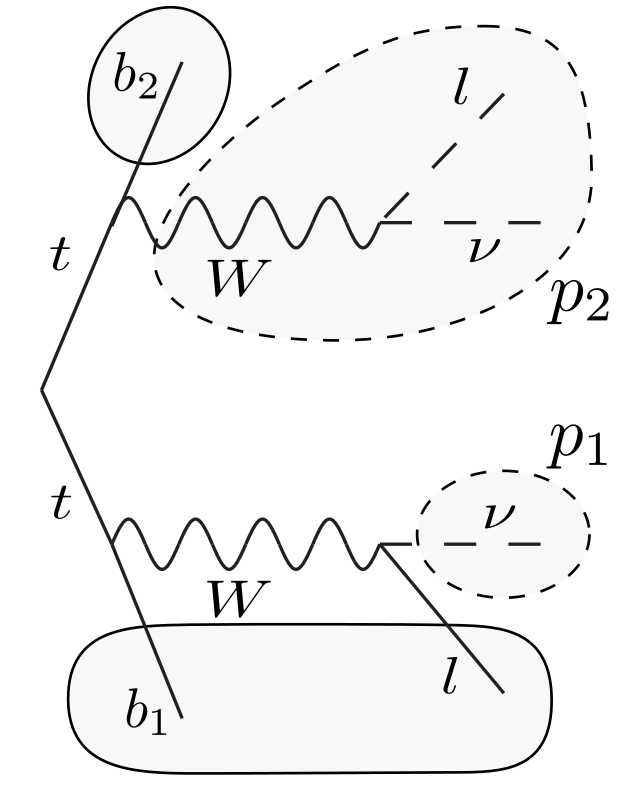
\includegraphics[width=0.33\linewidth]{Figures/mt2w_sketch.png}
\caption{\label{fig:mt2w_sketch}
Sketch of a dilepton \ttbar background event, dashed lines represent unseen
particles.}
\end{center}
\end{figure}

By cutting on a value larger than the top mass, this variable is very effective at removing the \ttbar lost lepton background.  Additionally, this variable has extended tails for signal hypotheses with large $\Delta$M between the stop and LSP.  Signal hypotheses with small $\Delta$M between the stop and LSP peak for masses smaller than the top mass.  Therefore, the search regions are classified into two types: \textit{High $\Delta$M} and \textit{Low $\Delta$M}, by cutting above and below a value just above the top mass. 

\begin{itemize}
  \item \textit{High $\Delta$M}: $\MTtW>200\GeV$
  \item \textit{Low $\Delta$M}: $\MTtW<200\GeV$
\end{itemize}


\subsubsection{ \MET}
\label{sec:obj_sel:met}

The \MET is calcuated as the vector sum of all PF candidates reconstructed in teh event.  The jet energy corrections described in section \ref{sec:obj_sel:jet_sel}.  

The LSP particles in the final state of the stop decay create additional \MET in the signal events.  This is one of the most powerful discriminanting variables in the search.  The signal regions are created from exclusive \MET bins beginning at $\MET>250\GeV$ in each of the \textit{High $\Delta$M} and \textit{Low $\Delta$M} classifications.  


\subsubsection{ Signal Region Definitions }
\label{sec:obj_sel:signal_regions}

A total of 9 signal regions are used in this search.  As described in section \ref{sec:obj_sel:met}, they are formed by creating exclusive \MET bins in the \textit{High $\Delta$M} and \textit{Low $\Delta$M} classifications.  They are listed below:

\begin{itemize}
  \item $nJets==3$, \textit{High $\Delta$M}: $\MTtW>200\GeV$
  \begin{itemize}
    \item $\MET>350 \GeV$
  \end{itemize}
  \item $nJets\ge4$, \textit{Low $\Delta$M}: $\MTtW<200\GeV$
  \begin{itemize}
     \item $250<\MET<325 \GeV$
     \item $\MET>325 \GeV$
  \end{itemize}
  \item $nJets\ge4$, \textit{High $\Delta$M}: $\MTtW>200\GeV$
  \begin{itemize}
     \item $250<\MET<350 \GeV$
     \item $350<\MET<450 \GeV$
     \item $\MET>450 \GeV$
  \end{itemize}
\end{itemize}

